\chapter{User Comfort Improvement}
One of the main goals of ReminisceMe is to get people to play a lot of games in order to be able to collect a lot of information. The more a person plays and the longer they keep coming back to the game the more detailed the analysis can be. It is also important that the users enjoy the game enough for them to talk about it and attract more users. In general, we can say that this project trades enjoyment for data about autobiographical memory. For that to be possible, we need the game to be enjoyable and the player to feel comfortable while playing. A lot of measures have been been put in place to make the whole experiment as good as possible.
\section{Mobile improvements}
Most of the people today access the internet on their mobile device more than they do on a laptop or desktop computer. In fact, the largest part of Facebook users are mobile users \cite{mobileusage}. Therefore, we can safely expect that a decent portion of our user base will be mobile users, playing while on transportation or during a break. Making the experience great for these players is then an important concern.
\subsubsection{Mobile application}
Up to now, the way to access ReminisceMe on a mobile device was through a browser on the phone. Some basic application had been tested in the past but it could not really be used as a replacement for the web application. The problems that come from using ReminisceMe on a mobile phone are the following:
\begin{enumerate}
	\item It uses a lot of bandwidth: there is a lot of data downloaded to get to the website, it is rarely a problem when using it with a proper wi-fi or cabled connection but becomes one when using the mobile network
	\item It has to use the same graphical instructions and code as the code running on a computer, it is therefore not trivial to make sure everything is compatible. Even though most of it can be the same, having a separate place for mobile code is easier and less error prone.
	\item Some features, such as the notifications, the Facebook login and the Facebook friends invitations do not behave correctly or do not work at all.
\end{enumerate}

We decided to create a mobile application. It is built


\subsubsection{No post ordering}
Despite having a responsive design on a mobile application, certain elements cannot be displayed properly and even look weird on a large screen. The main difficulty about displaying posts is that their length and content cannot predicted and some large posts (which are consequently also more interesting) cannot be rendered nicely inside an ordering item. The decision was therefore made to drop all the questions which would ask to reorder posts.
\section{Blacklist}
Even though some discomfort such as reading old posts from a time when the user was a lot younger and a lot less mature can be funny, we still need to make sure this discomfort does not exceed a certain level. While the application was being tested by different users, some users came across content related to people they did not wish to hear about or events they are not willing to think about.\\
There are two main problems with those questions. The first is tied to a person. Be it an ex partner or a dead relative, we all know people whose name suffices to bring back painful memories or sad feelings. While this is a really unfortunate situation and it might diminish our capacity to generate questions, we felt compelled to add the possibility for the user to ignore Facebook users they do not want any mention of on their game boards. The main reason behind this decision is that, depending on the relationship between a potential player and some of the people mentioned in the questions, the discomfort can be big enough for the user to not want to play the game again. Unfortunately, it is impossible for us to predict when such a situation might arise and we cannot do a lot preemptively (beside highlighting the blacklist button so that the user thinks about it before even starting to play), but we hope that having the ability to ignore people is sufficient to make users stay after encountering such a situation. Figure \ref{fig:blacklist} shows the interface where a user can edit its blacklist.\\
The second problem is related to a particular event and is linked more to the content of a post than to the a person reacting, commenting or being mentioned in it. This problem is still open at the moment as analyzing the content (text, title or image) to see if it is related to something as abstract as an event is not an easy problem and would require more advanced machine learning techniques.
\begin{figure}
\centering
{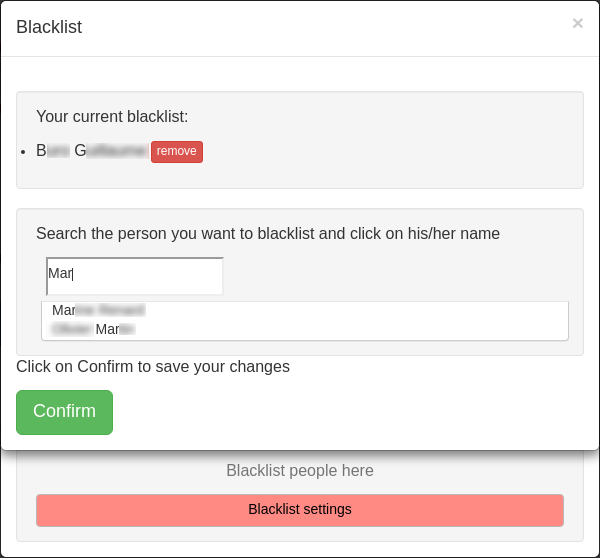
\includegraphics[width=3.5in]{images/blacklist.png}}
\caption{Blacklist Interface}
\label{fig:blacklist}
\end{figure}
\section{Notifications}